% ═════════════════════════════════════════════════════════════════════
% MAIN FIGURES
% ═════════════════════════════════════════════════════════════════════

\section{Main Figures}

\begin{figure}[H]
\centering
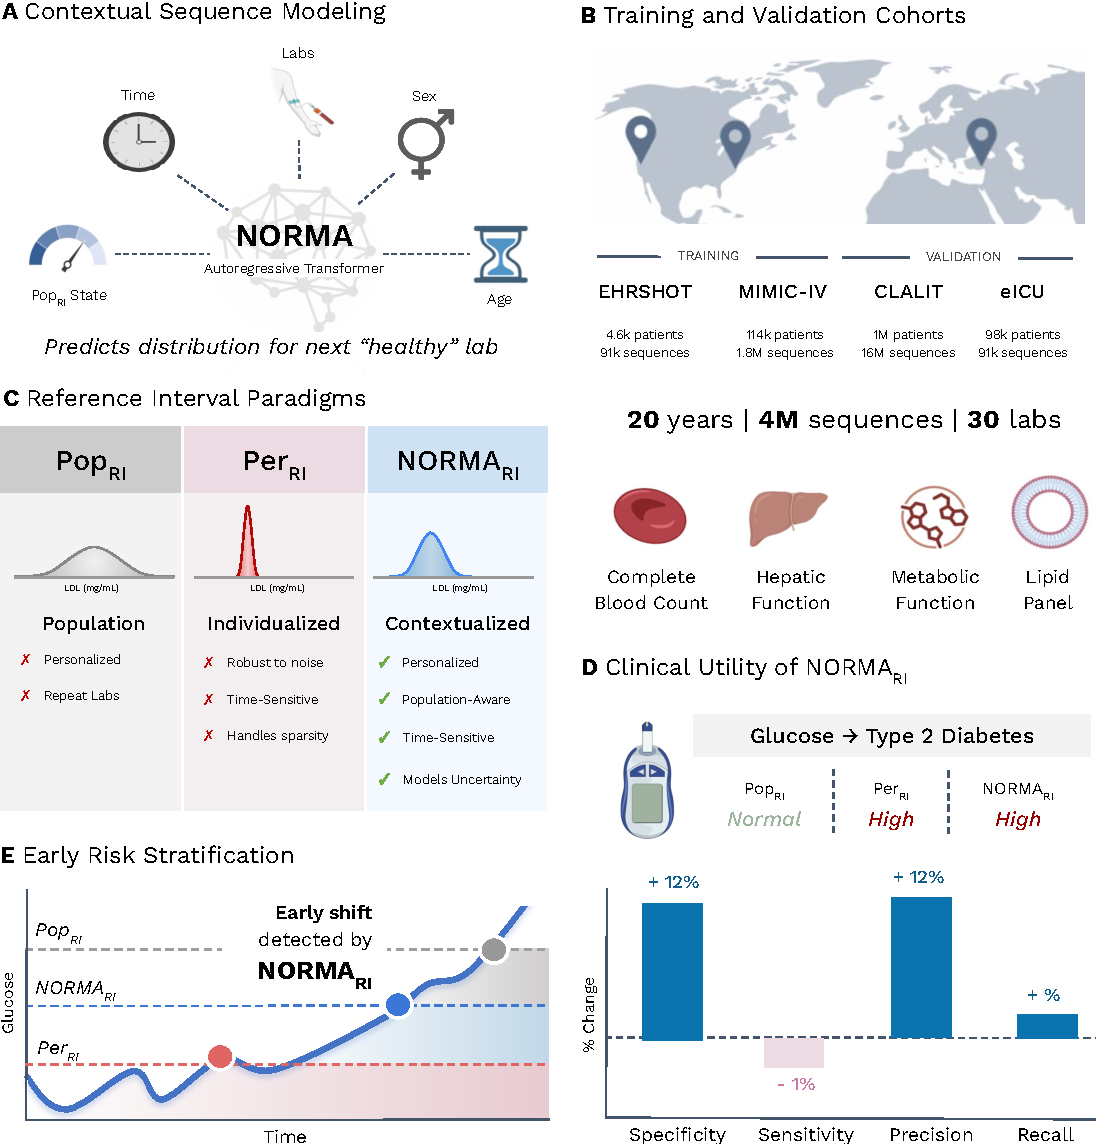
\includegraphics[width=\textwidth,height=0.78\textheight,keepaspectratio]{figures/figure1.pdf}
\caption{\textbf{Overview of NORMA.}
\textbf{(A)}~Contextual sequence modeling: NORMA is an autoregressive transformer that integrates labs, time, sex, age, and population-level state to predict the distribution of the next healthy lab value.
\textbf{(B)}~Training and validation cohorts spanning 20 years, 4M sequences, and 30 analytes across four datasets.
\textbf{(C)}~Reference interval paradigms: population (PopRI), individualized (PerRI), and contextualized (NORMA\textsubscript{RI}).
\textbf{(D)}~Clinical utility of NORMA\textsubscript{RI} for outcome prediction.
\textbf{(E)}~Early risk stratification via detection of shifts before population thresholds.}
\label{fig:figure1}
\end{figure}
\clearpage

\begin{figure}[H]
\centering
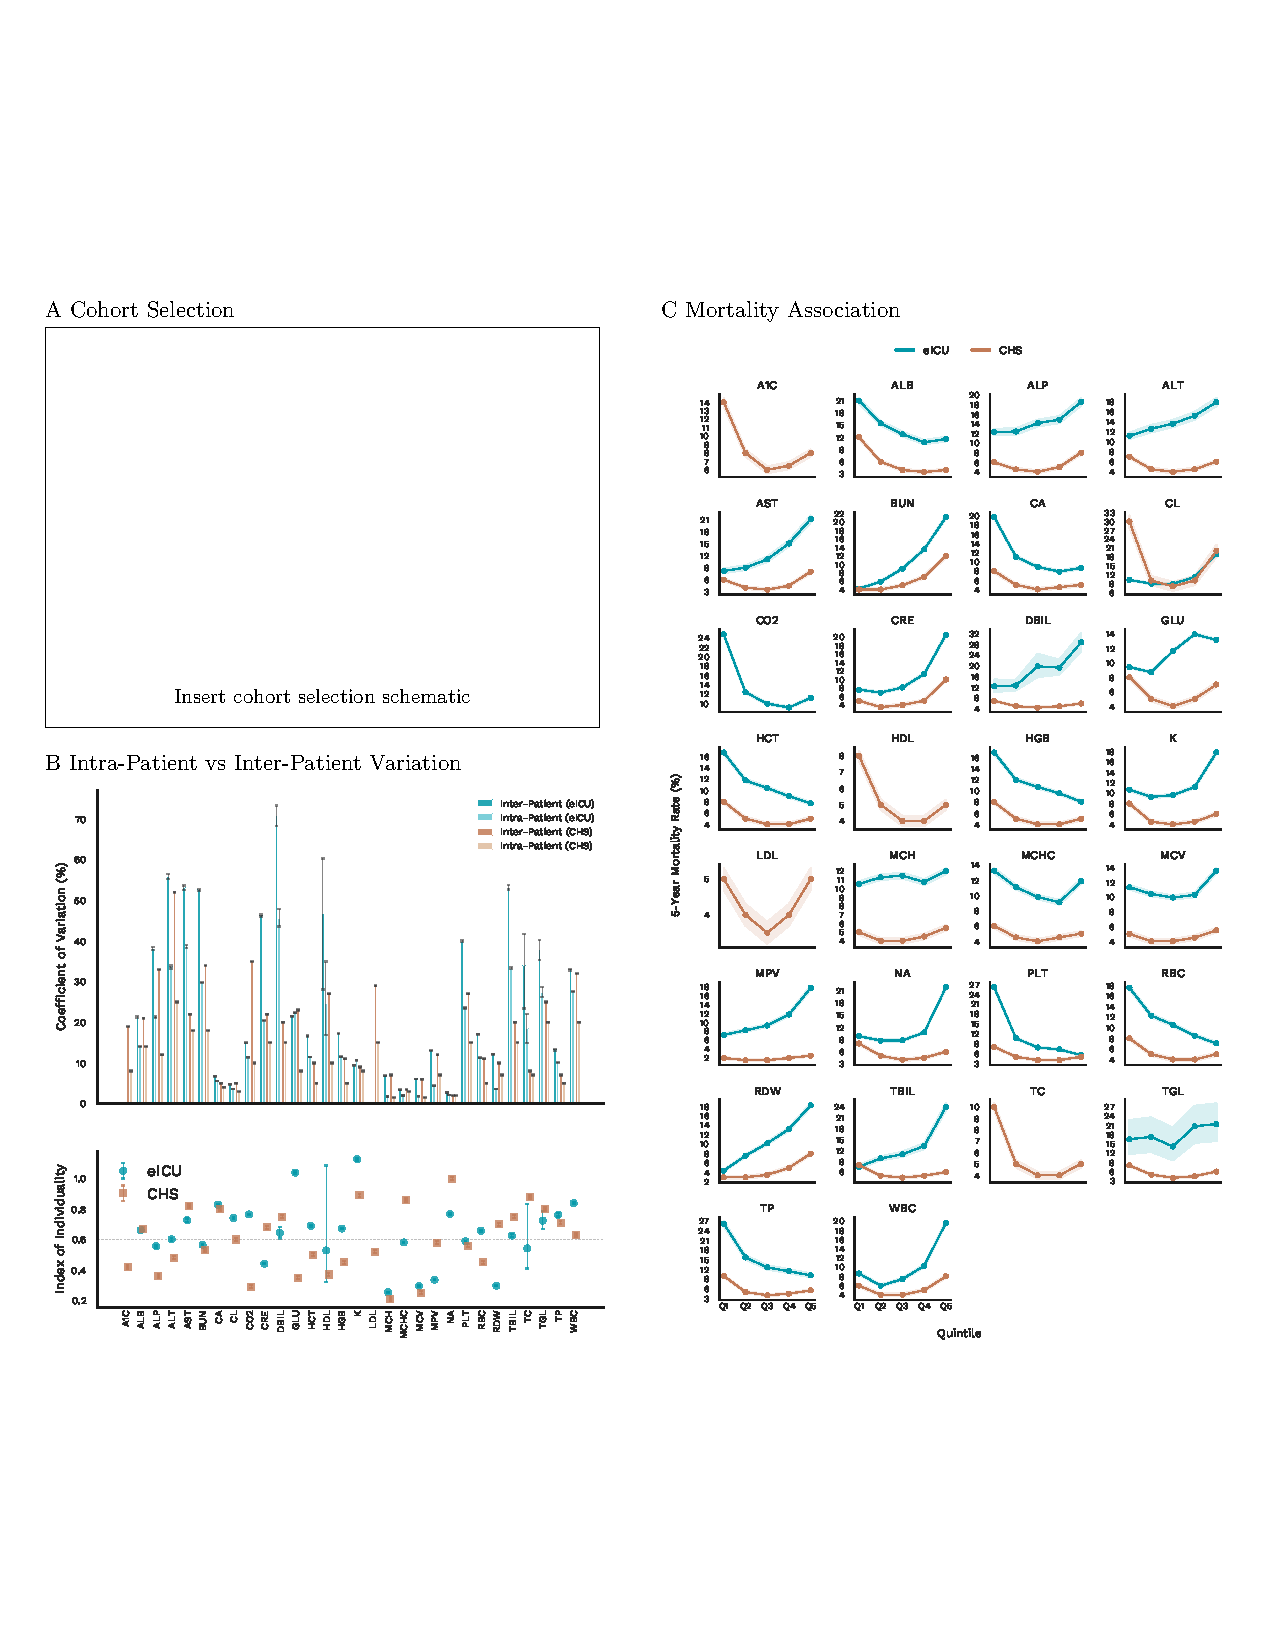
\includegraphics[width=\textwidth,height=0.78\textheight,keepaspectratio]{figures/figure2.pdf}
\caption{\textbf{Detection of within-person abnormalities by personalized intervals.}
\textbf{(A)}~Cohort selection schematic.
\textbf{(B)}~Intra-patient vs inter-patient coefficient of variation and index of individuality across 30 analytes.
\textbf{(C)}~Five-year mortality rate by quintile of raw analyte value for eICU and CHS cohorts.}
\label{fig:figure2}
\end{figure}
\clearpage

\begin{figure}[H]
\centering
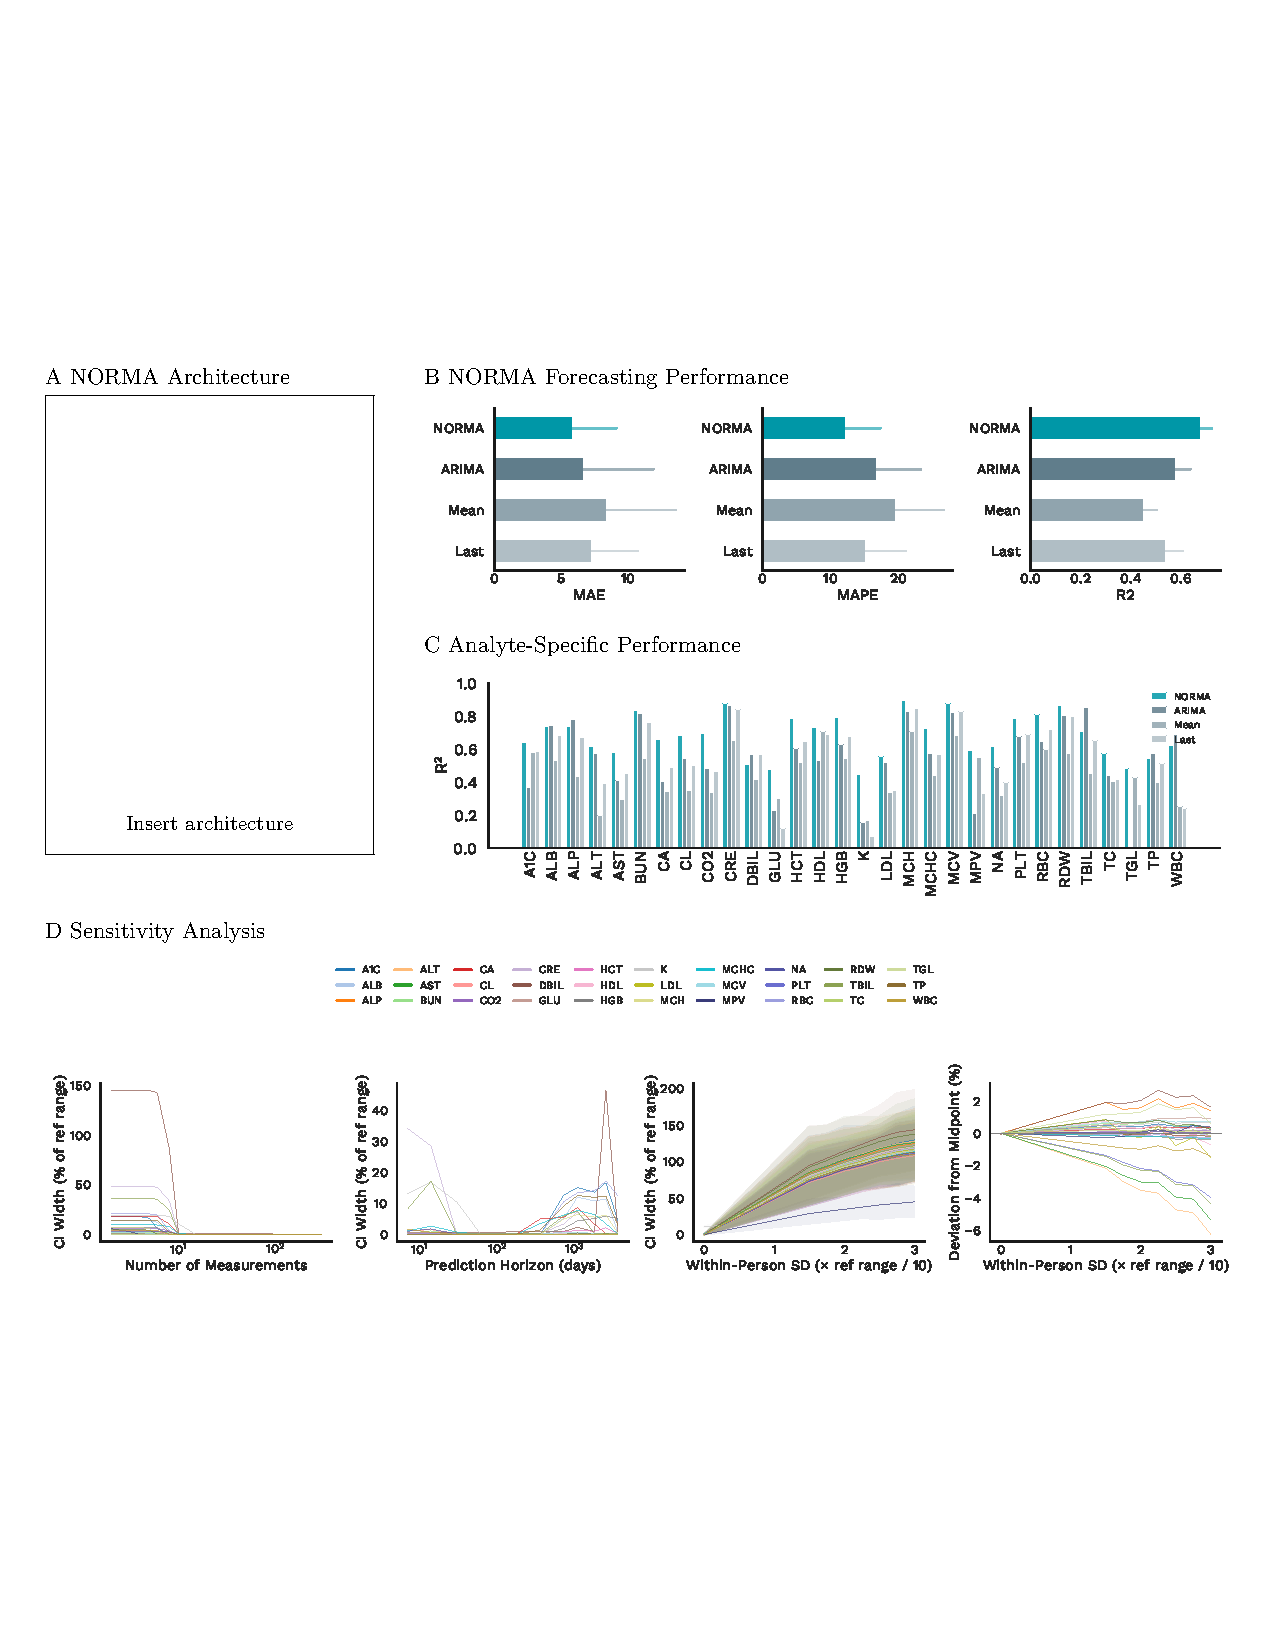
\includegraphics[width=\textwidth,height=0.78\textheight,keepaspectratio]{figures/figure3.pdf}
\caption{\textbf{NORMA architecture and predictive performance.}
\textbf{(A)}~Model architecture: decoder-only transformer with context, history, and query tokens producing quantile predictions.
\textbf{(B)}~Forecasting accuracy (MAE, MAPE, R\textsuperscript{2}) compared with ARIMA, patient mean, and last-value baselines.
\textbf{(C)}~Per-analyte R\textsuperscript{2} across 30 laboratory tests.
\textbf{(D)}~Sensitivity analysis: effect of history length, prediction horizon, and within-person variability on prediction interval width.}
\label{fig:figure3}
\end{figure}
\clearpage

\begin{figure}[H]
\centering
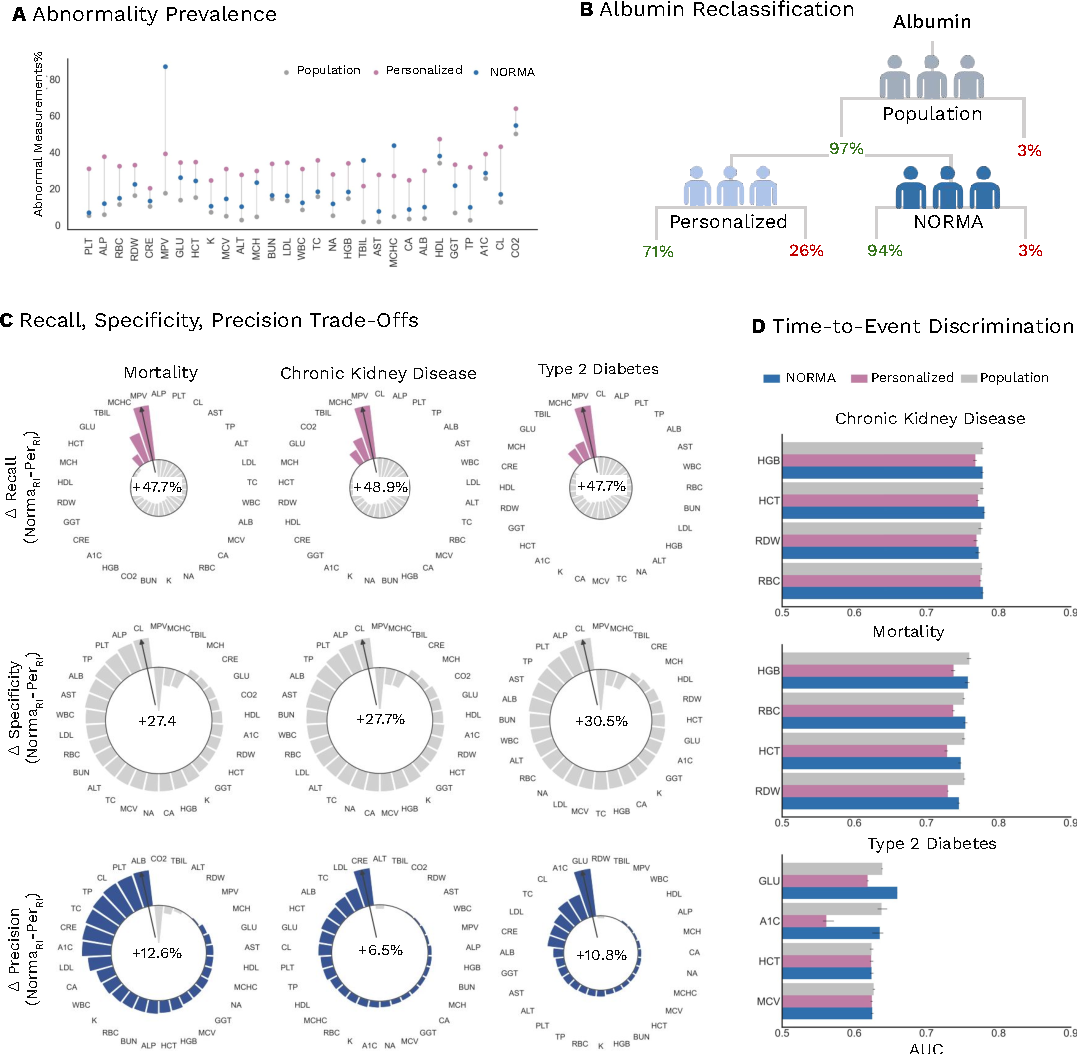
\includegraphics[width=\textwidth,height=0.78\textheight,keepaspectratio]{figures/figure4.pdf}
\caption{\textbf{Time-dependent discrimination for clinical outcomes in Clalit Health Services.}
\textbf{(A)}~Abnormality prevalence across reference interval frameworks (PopRI, PerRI, NORMA\textsubscript{RI}).
\textbf{(B)}~Albumin reclassification across paradigms.
\textbf{(C)}~Recall, specificity, and precision trade-offs (circos plots) for mortality, CKD, and type 2 diabetes.
\textbf{(D)}~Time-to-event discrimination (AUC) by analyte and method.}
\label{fig:figure4}
\end{figure}
\clearpage

\begin{figure}[H]
\centering
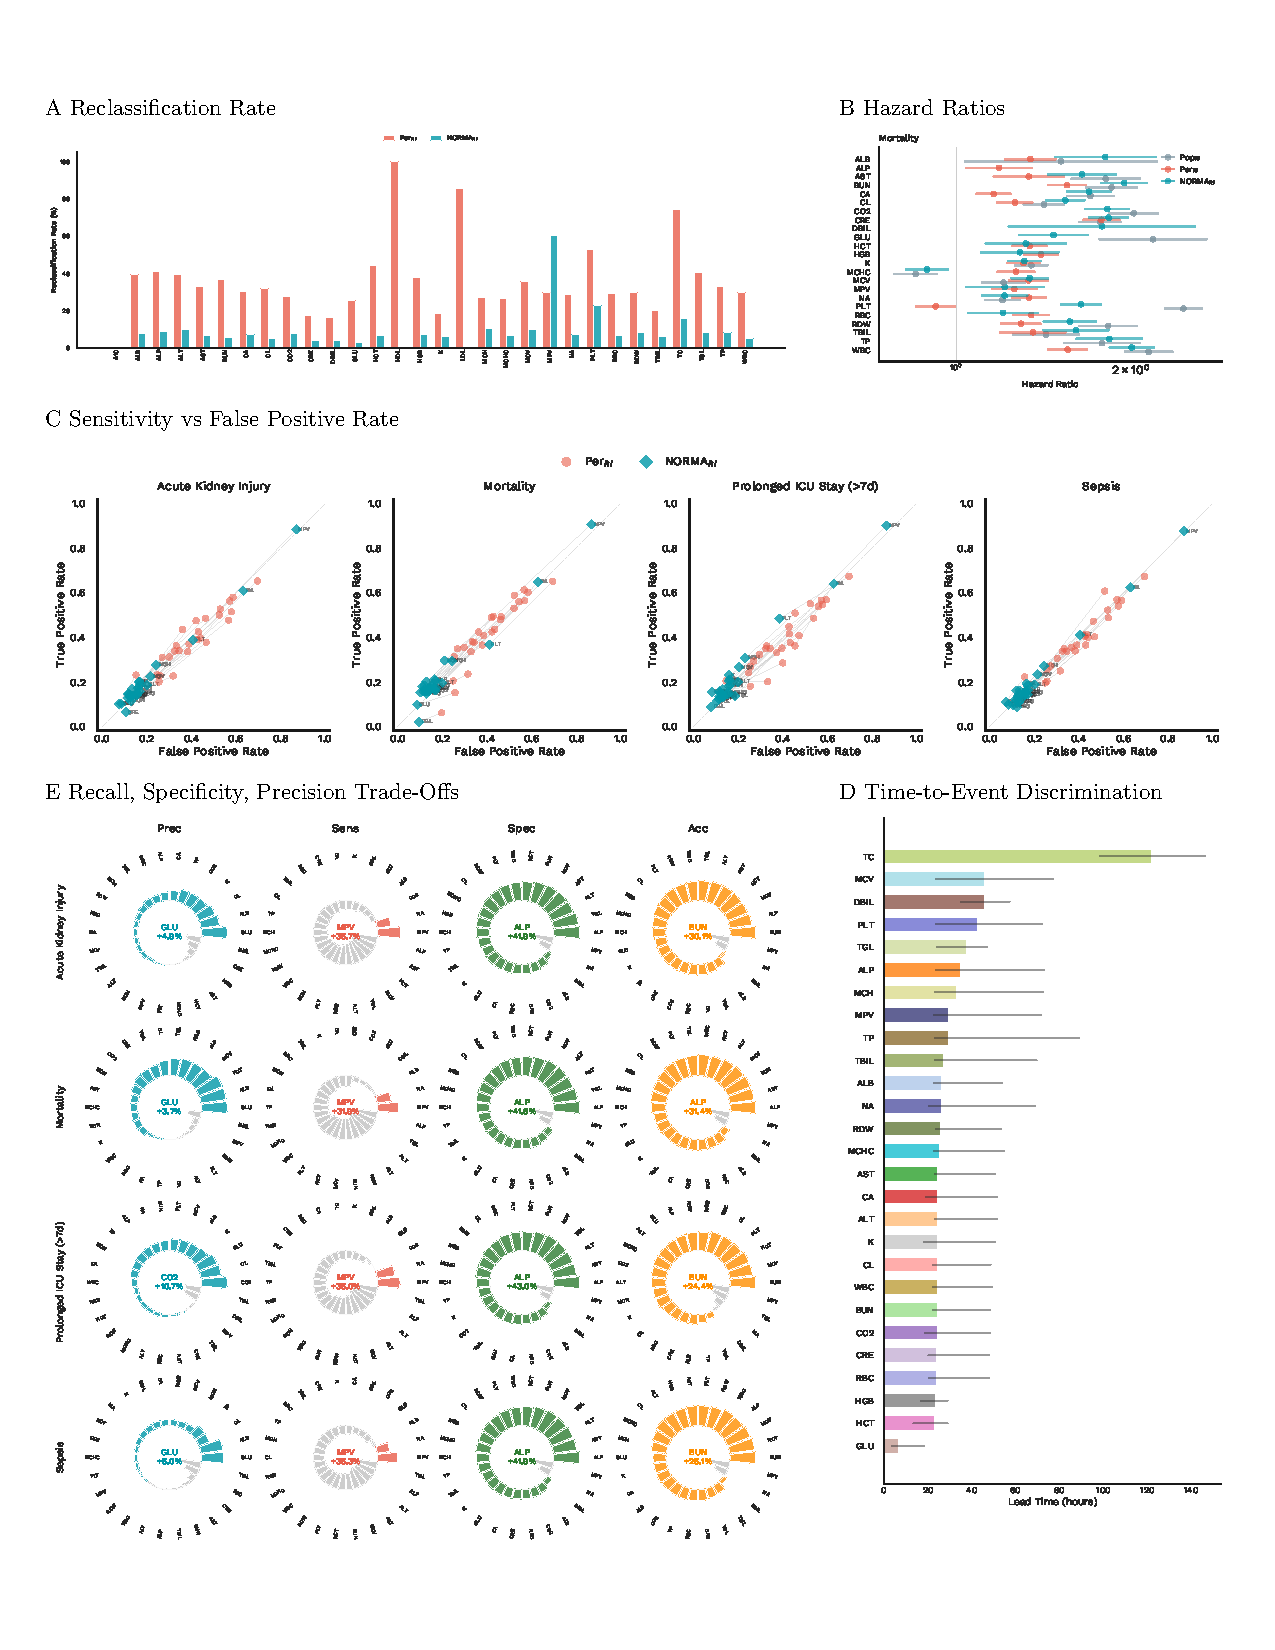
\includegraphics[width=\textwidth,height=0.78\textheight,keepaspectratio]{figures/figure5.pdf}
\caption{\textbf{Clinical outcome prediction in eICU.}
\textbf{(A)}~Reclassification rate among PopRI-normal measurements by PerRI and NORMA\textsubscript{RI}.
\textbf{(B)}~Cox proportional hazard ratios for mortality (significant associations only).
\textbf{(C)}~Sensitivity vs false positive rate for acute kidney injury, mortality, prolonged ICU stay, and sepsis.
\textbf{(D)}~Lead time: how much earlier NORMA flags abnormalities compared with PopRI.
\textbf{(E)}~Recall, specificity, precision, and accuracy trade-offs by outcome.}
\label{fig:figure5}
\end{figure}
\clearpage
